\documentclass[12pt,a4paper,french]{article}

\usepackage[utf8]{inputenc}
\usepackage[T1]{fontenc}
\usepackage{lmodern}
%\usepackage{fourier}

\usepackage[margin=1.4cm]{geometry}
\usepackage{titling}
\usepackage{amsmath,amsfonts,amssymb,amsthm}
\usepackage{tikz}
\usepackage{tkz-base}
\usetikzlibrary{intersections}
\usepackage{tabularx}
\usepackage{esvect}
\usepackage{delimset}

\usepackage{enumitem}
\setlist{noitemsep}
%\setlist[1]{\labelindent=\parindent} % < Usually a good idea
\setlist[itemize]{leftmargin=*}
\setlist[itemize,1]{label=$\triangleright$}
\setlist[enumerate]{labelsep=*, leftmargin=1.5pc}
\setlist[enumerate,1]{label=\textbf{\arabic*.}, ref=\arabic*}
\setlist[enumerate,2]{label=\emph{\alph*}),
ref=\theenumi.\emph{\alph*}}
\setlist[enumerate,3]{label=\roman*), ref=\theenumii.\roman*}
\setlist[description]{font=\sffamily\bfseries}

\usepackage{exsheets}
\usepackage{numprint}
\newcommand{\np}{\numprint}
\usepackage{tabularx}

\usepackage[pdfusetitle]{hyperref}

\usepackage{babel}

\newcommand{\N}{\mathbf{N}}
\newcommand{\norme}[1]{\left\lVert #1 \right\rVert}
%\newcommand{\abs}[1]{\left\lvert #1 \right\rvert}
\renewcommand{\u}{(u_n)_{n\in\N}}

\author{Vincent-Xavier \bsc{Jumel}}
\title{Terminale S, chapitre 1 : récurrence et suites}
\date{septembre 2017}

\setlength{\parindent}{0pt}
\everymath{\displaystyle}

\SetupExSheets{solution/print=false}


\begin{document}

\maketitle

\section{Raisonnement par récurrence}

\begin{question}[subtitle={Récurrence}]
  Démontrer par récurrence que, pour tout nombre entier naturel $n \geqslant
  6$, $2^n \geqslant 6n + 7$
\end{question}
\begin{solution}
  On considère la proposition $P_n$ : «$2^n \geqslant 6n + 7$».

  \emph{Initialisation} : Pour $n = 6$, d'une part $2^6 = 64$ et d'autre
  part, $6 \times 6 + 7 = 43$ donc $P_0$ est vraie.

  \emph{Hérédité} : Supposons que $P_n$ est vrai au rang $n$ arbitrairement
  choisi et montrons alors que $P_{n+1}$ est vraie.
  \begin{align*}
             & 2^n \geqslant 6n + 7                                \\
    \implies & 2^{n+1} \geqslant 12n + 7                           \\
    \implies & 2^{n+1} \geqslant 6n + 6 + 6n + 1 = 6(n+1) + 6n + 1 \\
    \implies & 2^{n+1} \geqslant 6(n+1) + 37 > 6(n+1) + 7 \qed
  \end{align*}

  \emph{Conclusion} : La propriété est vraie pour $n = 6$ et $P_n \implies
  P_{n+1}$ donc pour tout nombre entier naturel $n \geqslant 6$, $2^n
  \geqslant 6n + 7$.
\end{solution}

\begin{question}[subtitle={Récurrence encore}]
  Démonter par récurrence que, pour tout entier naturel $n$, $5^{n+2}
  \geqslant 4^{n+2} + 3^{n+2}$.
\end{question}
\begin{solution}
  On considère la proposition $P_n$ : «$5^{n+2} \geqslant 4^{n+2} + 3^{n+2}$».

  \emph{Initialisation} : Pour $n = 0$, c'est le «premier triplet de
  Pythagore» : $5^2 = 4^2 = 3^2$, donc la proposition est vraie au rang $n =
  0$.

  \emph{Hérédité} : Supposons que $P_n$ est vrai au rang $n$ arbitrairement
  choisi et montrons alors que $P_{n+1}$ est vraie.
  \begin{align*}
             & 5^{n+2} \geqslant 4^{n+2} + 3^{n+2}                            \\
    \implies & 5^{n+2} \times 5 \geqslant 4^{n+2} \times 5 + 3^{n+2} \times 5 \\
    \implies & 5^{n+3} \geqslant 4^{n+2} \times 4 + 3^{n+2} \times 3          \\
    \implies & 5^{n+3} \geqslant 4^{n+3} + 3^{n+3} \qed
  \end{align*}
  La majoration repose essentiellement sur le fait que $5 > 4$ et donc $a
  \times 5 > a \times 4$ pour tout $a > 0$, avec ici $a$ qui n'est autre que
  $4^{n+2}$ ou $3^{n+2}$.

  \emph{Conclusion} : La propriété est vraie pour $n = 0$  et $P_n \implies
  P_{n+1}$ donc pour tout nombre entier naturel $n$ $5^{n+2} \geqslant
  4^{n+2} + 3^{n+2}$.
\end{solution}

\begin{question}
  $P_n$ est la propriété : « $4^n + 1 $ est un multiple de 3», où $n$
  désigne un entier naturel.
  \begin{enumerate}
    \item Démontrer que, pour tout entier naturel $k$, si $P_k$ est vraie,
      alors $P_{k+1}$ est vraie.
    \item Que peut-on conclure ?
  \end{enumerate}
\end{question}
\begin{solution}
  \begin{enumerate}
    \item
      Soit $k$ un entier naturel. On suppose que $4^k + 1$ est un multiple
      de 3, c'es-à-dire qu'il existe un entier naturel $m$ tel que $4^k + 1
      = 3m$ ou encore que $4^k = 3m - 1$.

      Multiplions à droite et à gauche par 4 et on obtient $4^{k+1} = (3m -
      1) \times 4 = 12m - 4 = 3\times 4m - 3 - 1 = 3(4m - 1) - 1$. En
      résumé, on vient de trouver un entier $m'$ tel que $4^{k+1} = 3m' - 1$
      ce qui s'écrit aussi $4^{k+1} + 1 = 3m'$. Autrement dit, $4^{k+1} +
      1$ est un multiple de 3.
    \item On ne peut rien conclure. En effet, la proposition n'est pas
      initialisée (et ne s'initialise pour aucune valeur de $n$) et donc la
      proposition est fausse.
  \end{enumerate}
\end{solution}

\begin{question}
  Démontrer par récurrence que, pour tout nombr eentier naturel $n$, $0 +
  1^2 + 2^2 + \cdots + n^2 = \frac{n(n+1)(2n+1)}6$.
\end{question}
\begin{solution}
  Reprendre l'exemple du cours. La difficulté réside dans la factorisation :
  \begin{align*}
    \frac{n(n+1)(2n+1)}6 + (n+1)^2 & = (n+1) \frac{n(2n+1)}6 + (n+1) \frac{6(n+1)}6 \\
                                   & = (n+1) \frac{2n^2 + 7n + 6}6 \\
                                   & = (n+1) \frac{(n+2)(2n+3)}6 \qed
  \end{align*}
\end{solution}

\begin{question}
  $t$ est la suite définie par $t_0 = 0$ et pour tout nombre entier naturel
  n, \[ t_{n+1} = t_n + \frac1{(n+1)(n+2)} . \]
  \begin{enumerate}
    \item Écrire $t_1, t2, t_3$ sous forme de fractions irréductibles.
    \item Émettre une conjecture srur l'expression de $t_n$ sous la forme
      d'une fraction.
    \item Démontrer par récurrence l'expression de $t_n$ conjecturée.
  \end{enumerate}
\end{question}
\begin{solution}
  \begin{enumerate}
    \item $t_1 = \frac12 ; t_2 = \frac23 ; t_3 = \frac34$
    \item Quelques essais supplémentaires laissent penser que $t_n =
      \frac{n}{n+1}$
    \item Démontrons ce résultat par récurrence.

      \emph{Initialisation} : pour $n = 0$, le résultat est démontré.

      \emph{Hérédité} : supposons que pour $n$ fixé, $t_n =
      \frac{n}{n+1}$ et calculons $t_{n+1}$.
      \begin{align*}
        t_{n+1} & = t_n + \frac1{(n+1)(n+2)}           \\
                & = \frac{n}{n+1} + \frac1{(n+1)(n+2)} \\
                & = \frac{n(n+2) + 1}{(n+1)(n+2)}      \\
                & = \frac{n^2 + 2n + 1}{(n+1)(n+2)}    \\
                & = \frac{(n + 1)^2}{(n+1)(n+2)}       \\
                & = \frac{n+1}{n+2} \qed
      \end{align*}
      \emph{Conclusion} : La récurrence étant initialisée et l'hérédité
      étant démontrée, on a donc la conclusion : \[ \forall n \in \N, t_n =
      \frac{n}{n+1} . \]
  \end{enumerate}
\end{solution}

\section{Limites de suites}

\subsection{Limites de suites}

\begin{question}
  Donner la limite de la suite $(u_n)$ dans les cas suivants.
  \begin{enumerate}
    \item $u_n = n^2 + 3n - 1$
    \item $u_n = 3n^2 - 5n + 2$
    \item $u_n = \sqrt{n} - n$
    \item $u_n = \frac{1}{n^2 - 9}$
    \item $u_n = \frac{n^2 + 1}{n +3}$
    \item $u_n = \frac{n^2 - n}{n^3 + n}$
  \end{enumerate}
\end{question}
\begin{solution}
  \begin{enumerate}
    \item $\lim_{n \to +\infty} u_n = +\infty$ : par somme des limites.
    \item $\lim_{n \to +\infty} u_n = +\infty$ : on factorise par $n^2$ et
      pour tout $n$, $u_n = n^2\left(3 - \frac5n + \frac2{n^2}\right)$.
    \item $\lim_{n \to +\infty} u_n = - \infty$ : on factorise par
      $\sqrt{n}$ et pour tout $n$, $u_n = \sqrt{n} \left( \frac{1}{\sqrt{n}}
      - \sqrt{n} \right)$.
    \item $\lim_{n \to +\infty} u_n = 0$ : par inverse d'une limite.
    \item $\lim_{n \to +\infty} u_n = +\infty$ : on factorise par $n$ au
      numérateur et au dénominateur et pour tout $n$, $u_n = \frac{n \left(
      n + \frac{1}{n} \right)}{n \left( 1 + \frac{3}n \right)} $.
    \item $\lim_{n \to +\infty} u_n = 0$ : on factorise par $n^2$ au
      numérateur et au dénominateur et pour tout $n$, $u_n = \frac{n^2
      \left( 1 - \frac{1}n \right)}{n^2 \left(n + \frac1n \right)}$.
  \end{enumerate}
\end{solution}

\begin{question}
  Donner la limite de la suite $(u_n)$ dans les cas suivants.
  \begin{enumerate}
    \item $u_n = 10(1- (0,1)^n)$
    \item $u_n = \left( 1 + \frac1{100000}\right)^n$
    \item $u_n = \frac{1+ 4^n}{3 + 0,5^n}$
    \item $u_n = \frac{0,2^n - 1}{0,3^n + 1}$
  \end{enumerate}
\end{question}
\begin{solution}
  \begin{enumerate}
    \item $(0,1^n)$ est géométrique de raison inférieure à 1 en valeur
      absolue, donc elle converge vers 0 et $\lim_{n \to +\infty} u_n = 10$.
    \item Ici, la suite est géométrique de raison $>1$ donc la suite diverge
      vers $+\infty$.
    \item Le numérateur diverge vers $+\infty$ et le dénominateur est la
      somme d'une quantité finie et d'une suite qui converrge vers 0. Donc
      la limite est $+\infty$.
    \item En factorisant, on obtient, pour tout $n$ $u_n =
      \frac{0,2^n}{0,3^n}\left(\frac{ 1 - \frac{1}{0,2^n}}{1 +
      \frac{1}{0,3^n}} \right)$.

      $\lim_{n \to +\infty} \frac{ 1 - \frac{1}{0,2^n}}{1 + \frac{1}{0,3^n}}
      = 1$ et $\lim_{n \to +\infty} \frac{0,2^n}{0,3^n} = \lim_{n \to
      +\infty} \left(\frac23\right)^n = 0$. On a donc $\lim_{n \to +\infty}
      u_n = 0$.
  \end{enumerate}
\end{solution}

\begin{question}
  Une suite $u$ est telle que pour tout $n$ supérieur à 5 on a \[ 0
  \leqslant 1 - u_n \leqslant \left(\frac45\right)^n . \] Quelle est la
  lmite de $u$.
\end{question}
\begin{solution}
  La suite de terme général $\left(\frac45\right)^n$ est une suite
  géométrique de raison inférieure en valeur absolue à 1 donc elle converge
  vers 0.

  On en déduit que la suite de terme général $1 - u_n$ converge aussi vers 0
  et donc que la suite $u$ converge vers 1.
\end{solution}

\begin{question}
  Proposer une interprétation géométrique au résultat suivant : \[
  \frac12 + \frac14 + \frac18 + \frac1{2^n} = 1. \]
\end{question}

\subsection{Suites croissantes majorées}

\begin{question}
  On considère un triangle équilatéral, de côté 9cm. Soit le processus
  itératif suivant :
  \begin{itemize}
    \item découper un segment en 3 parties égales ;
    \item retirer la partie centrale ;
    \item remplacer la partie centrale par deux segments de même longueurs
      orientés vers l'extérieur ;
  \end{itemize}
  Avec ce processus, un segment est transformé de la façon suivante :

  \begin{center}
    \tikz{\draw (0,0) -- (6,0) ;} $\rightarrow$ \tikz{ \draw(0,0) -- (2,0) --
    (3,1.732) -- (4,0) -- (6,0) ; }
  \end{center}
  \begin{enumerate}
    \item Tracer le triangle initial et les deux premières itérations.
    \item Donner l'expression du périmètre de la figure. En déduire que
      celui-ci diverge vers $+\infty$ (on pourra considérer la suite $(p_n)$
      des périmètres.)
    \item Justifier par un argument géométrique que l'aire de la figure est
      bornée et donner la borne supérieure.
    \item On considère la suite des aires, notée $(a_n)$. Proposer une
      expression de la forme $a_{n+1} = f(a_n)$.
  \end{enumerate}
\end{question}

\begin{question}
  On considère la suite $u$ définie par $u_0 \in \brk[s]*{\frac13 ; \frac23}$
  et pour tout entier naturel $n, u_{n+1} = \sqrt{3u_n - 1}$.
  \begin{enumerate}
    \item Démontrer que la suite $u$ est croissante.
    \item Justifier que la suite est convergente.
    \item Démontrer que si la suite converge vers $\ell$ alors $\ell = 1$ ou
      0.
    \item Déterminer la limite de $u_n$.
  \end{enumerate}
\end{question}

\begin{question}
  Soit $(u_n)_{n\in\N}$ la suite définie par $u_0 = 5$ et pour tout
  nombre entier naturel $n$, par \[u_{n+1} = \frac{4u_n - 1}{u_n+2}.\]
  Si $f$ est la fonction définie sur l'intervalle $]-2;+\infty[$ par \[
  f(x) = \frac{4x -1}{x+2}, \] alors on a pour tout entier naturel,
  $u_{n+1} = f(u_n)$. On donne en annexe une partie de la courbe
  $\mathcal{C}_f$ de la courbe de la fonction $f$ ainsi que la droite
  $\delta$ d'équation $y=x$.

  \begin{enumerate}
    \item \begin{enumerate}
      \item Sur l'axe des abscisses, placer $u_0$ puis construire
        $u_1$, $u_2$ et $u_3$ en laissant apparents les traits de
        construction.
      \item Quelles conjectures peut-on emettre sur le sens de
        variation et sur la convergence de la suite $(u_n)_{n\in\N}$ ?
    \end{enumerate}
  \item \begin{enumerate}
    \item Démontrer par récurrence que, pour tout nombre entier
      naturel, $\ u_n -1 > 0$.

    \item \emph{Dans cette question toute trace de recherche, même
        incomplète ou d'initiative même non fructueuse sera prise en
      compte dans l'évaluation.}

      Valider par une démonstration les conjectures émises à la
      question 1.b)
  \end{enumerate}
\item Dans cette question, on se propose d'étudier la suite
  $(u_n)_{n\in\N}$ par une autre méthode, en déterminant une
  expression de $u_n$ en fonction de $n$.

  Pour tout nombre entier naturel, on pose \[ v_n = \frac1{u_n -1}.
  \]
  \begin{enumerate}
    \item Démontrer que la suite $(v_n)_{n\in\N}$ est une suite
      arithmétique de raison $\frac13$.

    \item Pour tout nombre entier naturel, exprimer $v_n$ puis $u_n$
      en fonction de $n$.

    \item En déduire la limite de la suite $(u_n)_{n\in\N}$.
  \end{enumerate}
  \end{enumerate}
  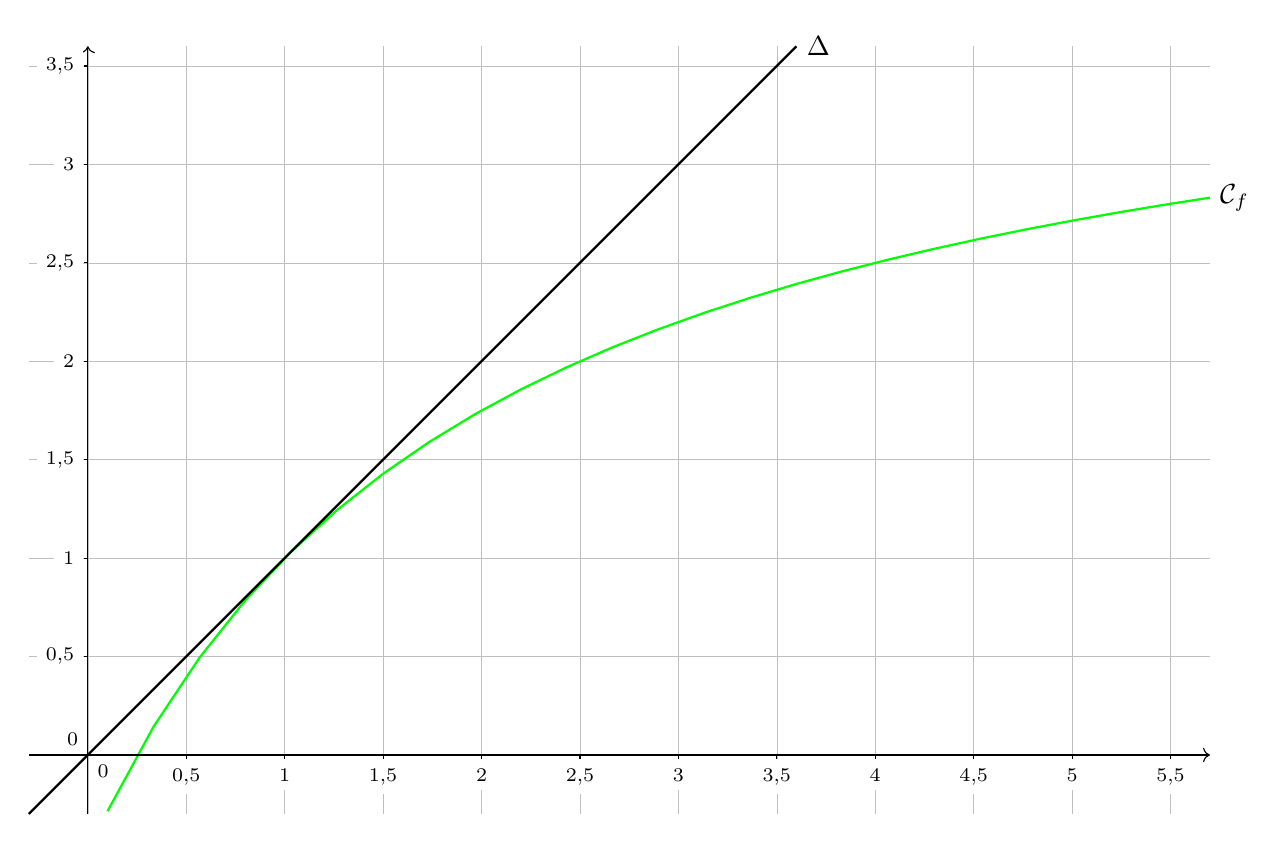
\begin{tikzpicture}[scale=2.5]
    \draw[very thin, lightgray] (-0.3,-0.3) grid [step=0.5] (5.7,3.6) ;
    \draw[thick,green] plot [domain=0.1:5.7] (\x,{(4*\x-1)/(\x+2)}) node
      [right,black] { $\mathcal{C}_f$ } ;
    \draw[thick] plot [domain=-0.3:3.6] (\x,\x) node[right] {
      $\Delta$ } ;
    \draw[->] (-0.3,0) -- (5.7,0) ; \draw [->] (0,-0.3) -- (0,3.6) ;
    \foreach \x in {0.5,1,...,5.5} {
      \draw (\x,0) -- (\x,-0.02) node [below,fill=white] {
        \scriptsize \np{\x} } ;
    }
    \foreach \y in {0.5,1,...,3.5} {
      \draw (0,\y) -- (-0.02,\y) node [left,fill=white] {
        \scriptsize \np{\y} } ;
    }
    \draw (0,0) node[below right] { \scriptsize 0} ;
    \draw (0,0) node[above left] { \scriptsize 0} ;
  \end{tikzpicture}
\end{question}
\begin{solution}
  \begin{enumerate}
    \item \begin{enumerate}
      \item cf Annexe.
      \item La suite $\u$ \emph{semble} être décroissante.
    \end{enumerate}
  \item \begin{enumerate}
    \item Démontrons par récurrence que $\forall n\in\N,\ u_n -1 >
      0$.

      \begin{description}
        \item[Initialisation] $u_0 = 5$ et $5 - 1 = 4 > 0$, donc la
          proposition est vraie au rang $n$.
        \item[Hérédité] Soit $n$ un entier naturel et supposons que
          $u_n-1 > 0$

          $u_n - 1 > 0 \implies u_n + 2 > 3 > 0$

          $u_{n+1} - 1 = \frac{4u_n -1}{u_n+2} - 1 = \frac{4u_n - 1
          - u_n -2}{u_n + 2} = \frac{3(u_n -1)}{u_n+2}$

          L'hypothèse de récurrence garantit que numérateur et
          dénominateur sont positifs, donc $\boxed{u_{n+1} -1 > 0}$.
        \item[Conclusion] $\forall n \in \N,\ u_n -1 >0$
      \end{description}
    \item Montrons que la suite est décroissante, c'est à dire que
      $\forall n \in \N,\ u_{n+1} \leqslant u_n$.

      Raisonnons par équivalences successives :

      $u_{n+1} = \frac{4u_n -1}{u_n+2} \leqslant u_n \iff 4u_n -1
      \leqslant u_n^2 + 2u_n \iff 0\leqslant u_n^2 - 2u_n +1 = (u_n
      -1)^2$. Cette dernière affirmation étant toujours vraie, on a
      la décroissance conjecturée.
  \end{enumerate}
    \item \begin{enumerate}
      \item Démontrons que $(v_n)_{n\in\N}$ est une suite
        arithmétique.

        $v_{n+1} - v_n = \frac1{u_{n+1}-1} - \frac1{u_n -1} =
        \frac{\frac13(u_n + 2)}{u_n -1 } - \frac1{u_n -1} =
        \frac{\frac13 u_n - \frac13}{u_n -1} = \frac13$.

        La suite est donc arithmétique de raison $\frac13$.

      \item $v_n = \frac13 n + \frac14$

        $u_n = \frac1{v_n} + 1 = 1 + \frac1{\frac13 n + \frac14}$

      \item $\boxed{\lim_{n\to+\infty} u_n = 1}$
    \end{enumerate}
\end{enumerate}


\vfill
\hfill
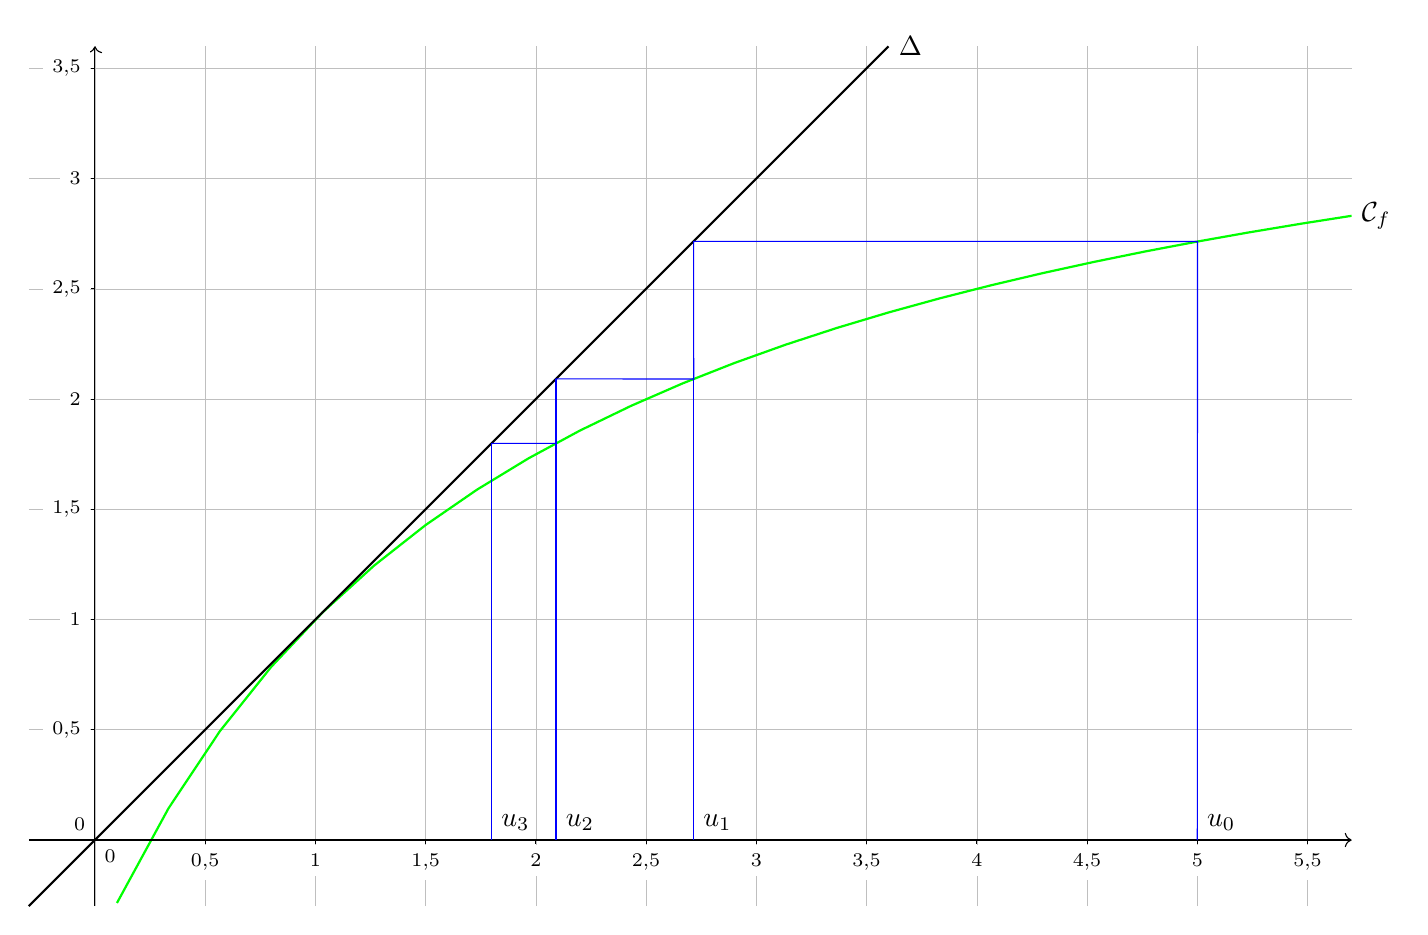
\begin{tikzpicture}[scale=2.8]
  \draw[very thin, lightgray] (-0.3,-0.3) grid [step=0.5] (5.7,3.6) ;
  \draw[thick,green,name path=f] plot [domain=0.1:5.7]
    (\x,{(4*\x-1)/(\x+2)}) node [right,black] { $\mathcal{C}_f$
    } ;
  \draw[thick,name path= D] plot [domain=-0.3:3.6] (\x,\x)
    node[right] { $\Delta$ } ;
  \draw[->] (-0.3,0) -- (5.7,0) ; \draw [->] (0,-0.3) -- (0,3.6) ;
  \foreach \x in {0.5,1,...,5.5} {
    \draw (\x,0) -- (\x,-0.02) node [below,fill=white] {
      \scriptsize \np{\x} } ;
  }
  \foreach \y in {0.5,1,...,3.5} {
    \draw (0,\y) -- (-0.02,\y) node [left,fill=white] {
      \scriptsize \np{\y} } ;
  }
  \draw (0,0) node[below right] { \scriptsize 0} ;
  \draw (0,0) node[above left] { \scriptsize 0} ;

  % construction réponse
  \newdimen\posy
  \newdimen\posx
  \path [name path = u0] (5,0) -- (5,3) ;
  \path [name intersections = {of = f and u0 }] ;
  \coordinate (A) at (intersection-1) ;
  \pgfextracty{\posy}{\pgfpointanchor{A}{center}}
  \path [name path=fu0] (A) -- (0,\posy) ;
  \path [name intersections = {of = fu0 and D}] ;
  \coordinate (B) at (intersection-1) ;
  \pgfextractx{\posx}{\pgfpointanchor{B}{center}}
  \draw[blue,name path=u1] (B) -- (\posx,0) node [above right,
    black] {$u_1$};
  \path [name intersections = {of = u1 and f}] ;
  \coordinate (C) at (intersection-1) ;
  \pgfextracty{\posy}{\pgfpointanchor{C}{center}}
  \path [name path = fu1] (C) -- (0,\posy) ;
  \path [name intersections = {of = fu1 and D}] ;
  \coordinate (D) at (intersection-1) ;
  \pgfextractx{\posx}{\pgfpointanchor{D}{center}}
  \draw[blue,name path=u2] (D) -- (\posx,0) node [above right,
    black] {$u_2$};
  \path [name intersections = {of = u2 and f}] ;
  \coordinate (E) at (intersection-1) ;
  \pgfextracty{\posy}{\pgfpointanchor{E}{center}}
  \path [name path=fu2 ] (E) -- (0,\posy) ;
  \path [name intersections = {of = fu2 and D}] ;
  \coordinate (F) at (intersection-1) ;
  \pgfextractx{\posx}{\pgfpointanchor{F}{center}}
  \draw[blue,name path=u3] (F) -- (\posx,0) node [above right,
    black] {$u_3$} ;


  \draw[blue] (5,0) node [above right,  black] {$u_0$} -- (A)
    -- (B) -- (C) -- (D) -- (E) -- (F) ;
\end{tikzpicture}
\end{solution}


\begin{question}
  On considère la suite $\left(u_n\right)$ définie par: 

  \[\left\{\begin{array}{l c l}
        u_0 &= &1 \quad  \text{et, pour tout entier naturel } n,\\
        \: u_{n+1} &=& \left(\dfrac{n+1}{2n+4}\right) u_n.
    \end{array}\right.\]

    On définit la suite $\left(v_n\right)$ par : pour tout entier naturel $n$,\: $v_n = (n + 1)u_n$.

    \medskip

    \parbox{0.55\linewidth}{\begin{enumerate}
        \item La feuille de calcul ci-contre présente les valeurs des
          premiers termes des suites $\left(u_n\right)$ et $\left(v_n\right)$, arrondies au cent-millième.

          Quelle formule, étirée ensuite vers le bas, peut-on écrire  dans la cellule B3 de la feuille de calcul pour obtenir les  termes successifs de $\left(u_n\right)$ ?
        \item  
          \begin{enumerate}
            \item Conjecturer l'expression de $v_n$ en fonction de $n$.
            \item Démontrer cette conjecture. 
          \end{enumerate}
        \item  Déterminer la limite de la suite $\left(u_n\right)$.
    \end{enumerate}} \hfill
    \parbox{0.42\linewidth}{
      \begin{tabularx}{\linewidth}{|c|*{3}{>{\centering \arraybackslash}X|}}\hline
        &A&B&C\\ \hline
        1 &$n$ 	&$u_n$ &$v_n$\\ \hline
        2 &0	& \np{1,00000}&\np{1,00000}\\ \hline
        3 &1 	& \np{0,25000} &\np{0,50000}\\ \hline
        4 &2	&\np{0,08333} &\np{0,25000}\\ \hline
        5 &3 	&\np{0,03125} &\np{0,12500}\\ \hline
        6 &4 	&\np{0,01250} &\np{0,06250}\\ \hline
        7 &5 	&\np{0,00521} &\np{0,03125}\\ \hline
        8 &6 	&\np{0,00223} &\np{0,01563}\\ \hline
        9 &7 	&\np{0,00098} &\np{0,00781}\\ \hline
        10 &8 	&\np{0,00043} &\np{0,00391}\\ \hline
        11 &9	&\np{0,00020} &\np{0,00195}\\ \hline
    \end{tabularx}}
\end{question}
\begin{solution}
  \begin{enumerate}
    \item Il faut écrire en B3 la formule \texttt{=(A2+1)/(2*A2+4)*B2}
\item  
	\begin{enumerate}
		\item %Conjecturer l'expression de $v_n$ en fonction de $n$.
On peut raisonnablement conjecturer que $v_n = \dfrac{1}{2^n}$ quel que soit $n \in \N$.
		\item %Démontrer cette conjecture. 
On a pour tout entier naturel $n$ :
		
$v_{n+1} = (n + 2)u_{n+1}$ et comme $u_{n+1} =\left(\dfrac{n+1}{2n+4}\right) u_n$, on peut écrire :
		
$v_{n+1} = (n + 2)\left(\dfrac{n+1}{2n+4}\right) u_n = (n + 2)\left(\dfrac{n+1}{2(n+2)}\right) u_n = \dfrac{n + 1}{2}u_n =  \dfrac{1}{2}\times (n + 1)u_n = \dfrac{1}{2}v_n$.

La relation $v_{n+1} = \dfrac{1}{2}v_n$, montre que la suite $\left(v_n\right)$ est une suite gémétrique de raison $\dfrac{1}{2}$ et de premier terme $v_0 = 1 \times u_0 = 1$.

On a donc pour tout entier naturel $n$, \: $v_n = \left(\dfrac{1}{2} \right)^n = \dfrac{1}{2^n}$.		
	\end{enumerate}
\item  %Déterminer la limite de la suite $\left(u_n\right)$.
Pour tout entier naturel $n$, \: $v_n = (n + 1)u_n \iff u_n = \dfrac{v_n}{n+1}$.

Or comme $-1 < \dfrac{1}{2} < 1$, on sait que $\displaystyle\lim_{n \to + \infty}\left(\dfrac{1}{2} \right)^n = 0$ et comme $\displaystyle\lim_{n \to + \infty}\dfrac{1}{n + 1} = 0$, on a par produit de limites :

\[\displaystyle\lim_{n \to + \infty} u_n = 0.\]
\end{enumerate}
\end{solution}

\newpage

\centering{\bfseries \Large \thetitle solutions }

\bigskip

\printsolutions

\end{document}
